% Latex template: mahmoud.s.fahmy@students.kasralainy.edu.eg
% For more details: https://www.sharelatex.com/learn/Beamer

\documentclass[aspectratio=1610]{beamer}					% Document class

\setbeamertemplate{footline}[text line]{%
  \parbox{\linewidth}{\vspace*{-8pt}A brief introduction to graphical models and deep methods in computational network biology \hfill\insertshortauthor\hfill\insertpagenumber}}
\setbeamertemplate{navigation symbols}{}

\usepackage[english]{babel}				% Set language
\usepackage[utf8x]{inputenc}			% Set encoding

\mode<presentation>						% Set options
{
  \usetheme{default}					% Set theme
  \usecolortheme{default} 				% Set colors
  \usefonttheme{default}  				% Set font theme
  \setbeamertemplate{caption}[numbered]	% Set caption to be numbered
}

% Uncomment this to have the outline at the beginning of each section highlighted.
%\AtBeginSection[]
%{
%  \begin{frame}{Outline}
%    \tableofcontents[currentsection]
%  \end{frame}
%}

\usepackage{graphicx}					% For including figures
\usepackage{booktabs}					% For table rules
\usepackage{hyperref}					% For cross-referencing
\usepackage[absolute,overlay]{textpos}
\usepackage{bm}

\title{Dynamics on gene networks}	% Presentation title
\author{Clayton W. Seitz}								% Presentation author
\date{\today}									% Today's date	

\begin{document}

% Title page
% This page includes the informations defined earlier including title, author/s, affiliation/s and the date
\begin{frame}
  \titlepage
\end{frame}

% Outline
% This page includes the outline (Table of content) of the presentation. All sections and subsections will appear in the outline by default.
\begin{frame}{Outline}
  \tableofcontents
\end{frame}

% The following is the most frequently used slide types in beamer
% The slide structure is as follows:
%
%\begin{frame}{<slide-title>}
%	<content>
%\end{frame}

\begin{frame}{Project Overview and Research Strategy}

\begin{textblock*}{7cm}(1cm,2cm)
\begin{figure}
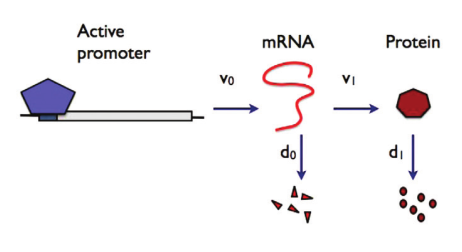
\includegraphics[width=7cm]{linear.png}
\caption{5-gene network sampled from \emph{Saccharomyces Genome Database} (SGD)}
\end{figure}
\end{textblock*}

\end{frame}

\begin{frame}{Training on BBBC039 U2OS Cells}
\vspace{0.1in}
BBBC039: 200 images, 160 train + 40 validation, 256\;x\;256 random crop

\begin{center}
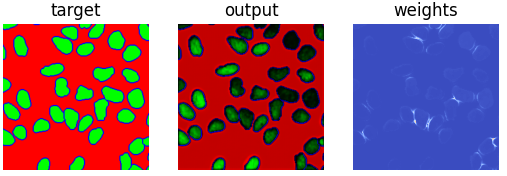
\includegraphics[width=0.8\textwidth]{weights.png}
\end{center}

We train a 3-channel semantic segmentation model with \textbf{weighted} cross-entropy loss:

\begin{equation*}
\mathcal{L} = \sum_{i,j} w_{ij}\log p_{ij}(\tilde{x}) = \sum_{i,j} w_{ij}\log \frac{\exp(-s_{ij}(\tilde{x}))}{\sum_{x\in\chi} \exp(-s_{ij}(\tilde{x}))}
\end{equation*}

$p_{ij}$ is the probability the model assigns a pixel to the true class $\tilde{x} \in \{\textrm{a}, \textrm{b}, \textrm{c}\}$

\end{frame}

\begin{frame}{Training on BBBC039 U2OS Cells}

\begin{center}
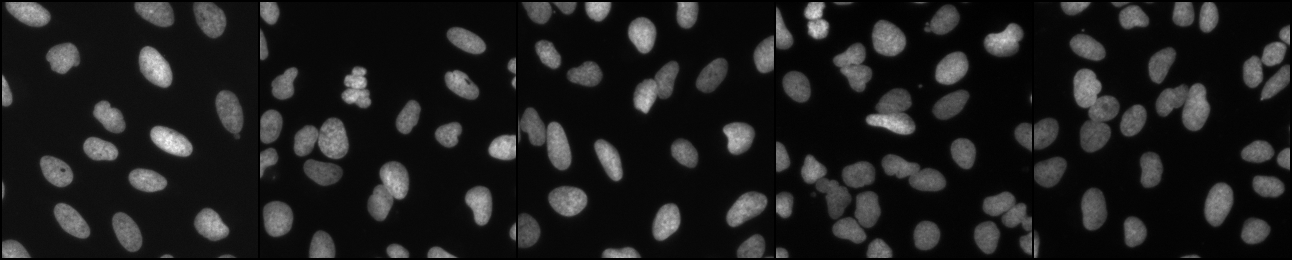
\includegraphics[width=0.85\textwidth]{input-train.png}
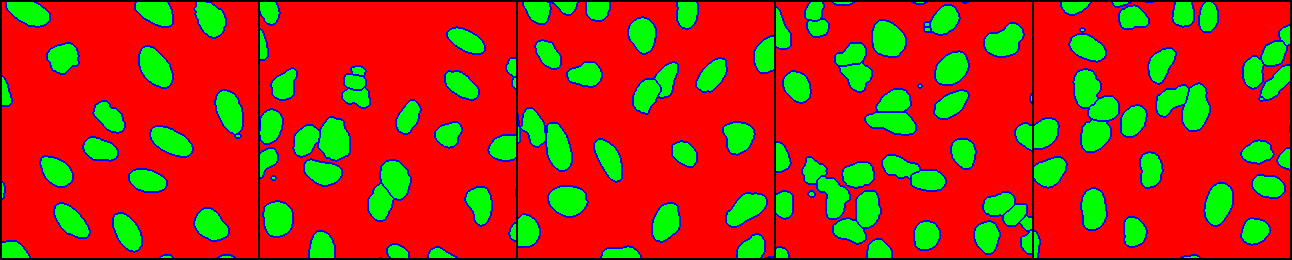
\includegraphics[width=0.85\textwidth]{target-train.png}
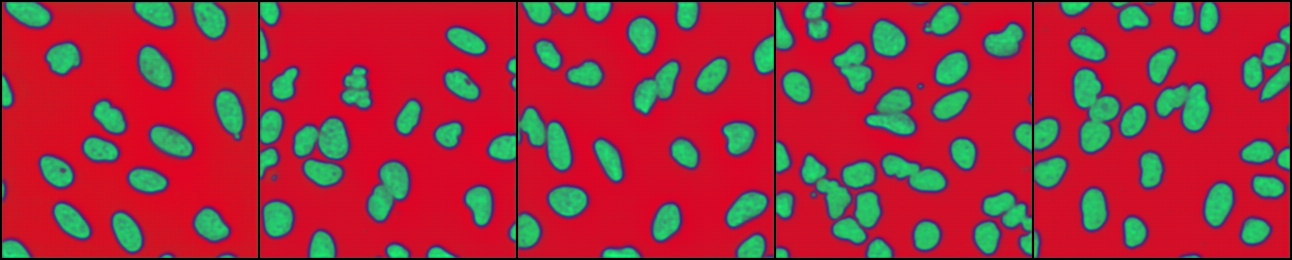
\includegraphics[width=0.85\textwidth]{output-train.png}
\end{center}

\end{frame}

\begin{frame}{Training on BBBC039 U2OS Cells}
Learning rate $\eta=0.01$, Batch-size $B=5$ (32 train iterations, 8 validation)
\begin{center}
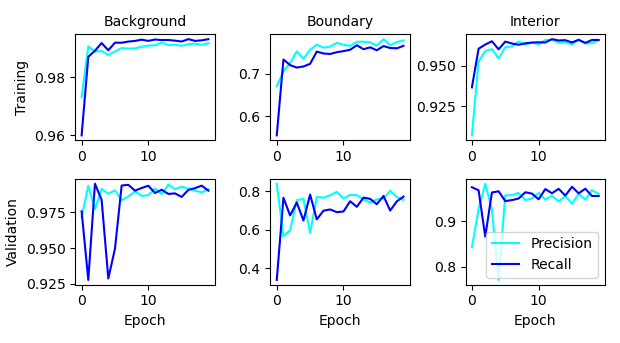
\includegraphics[width=0.85\textwidth]{metrics.png}
\end{center}

\end{frame}

\begin{frame}{Useful Algorithms for Data Processing}

1. Single Cell Variational Inference\\
2. Phi-Mixing Coefficient

\end{frame}

\begin{frame}{Models of transcription and translation}

\begin{textblock*}{5cm}(2cm,1.25cm)
\textbf{Linear Model}
\end{textblock*}

\begin{textblock*}{7cm}(0.35cm,1.25cm)
\begin{figure}
\begin{align*}
\dot{y_{i}} &= a_{i}x_{i} - b_{i}y_{i} + \xi_{i}\\
\dot{x_{i}} &= \sum_{j}m_{ij}y_{j} - c_{i}x_{i} + \eta_{i}
\end{align*}
\end{figure}
\end{textblock*}

\begin{textblock*}{5cm}(8cm,1.25cm)
\textbf{Nonlinear Model}
\end{textblock*}

\begin{textblock*}{7cm}(8cm,1.25cm)
\begin{figure}
\begin{align*}
\dot{y_{i}} &= a_{i}x_{i} - b_{i}y_{i} + \alpha_{i}\\
\dot{x_{i}} &= \sum_{j}m_{ij}\frac{y_{ij}^{n_{ij}}}{y_{ij}^{n_{ij}}+h_{ij}^{n_{ij}}} - c_{i}x_{i} + \beta_{i}
\end{align*}
\end{figure}
\end{textblock*}


\begin{textblock*}{7cm}(0.5cm,3.5cm)
\begin{figure}
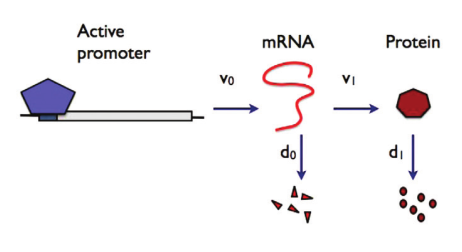
\includegraphics[width=7cm]{linear.png}
\caption{5-gene network sampled from \emph{Saccharomyces Genome Database} (SGD)}
\end{figure}
\end{textblock*}

\begin{textblock*}{7cm}(8cm,4cm)
\begin{figure}
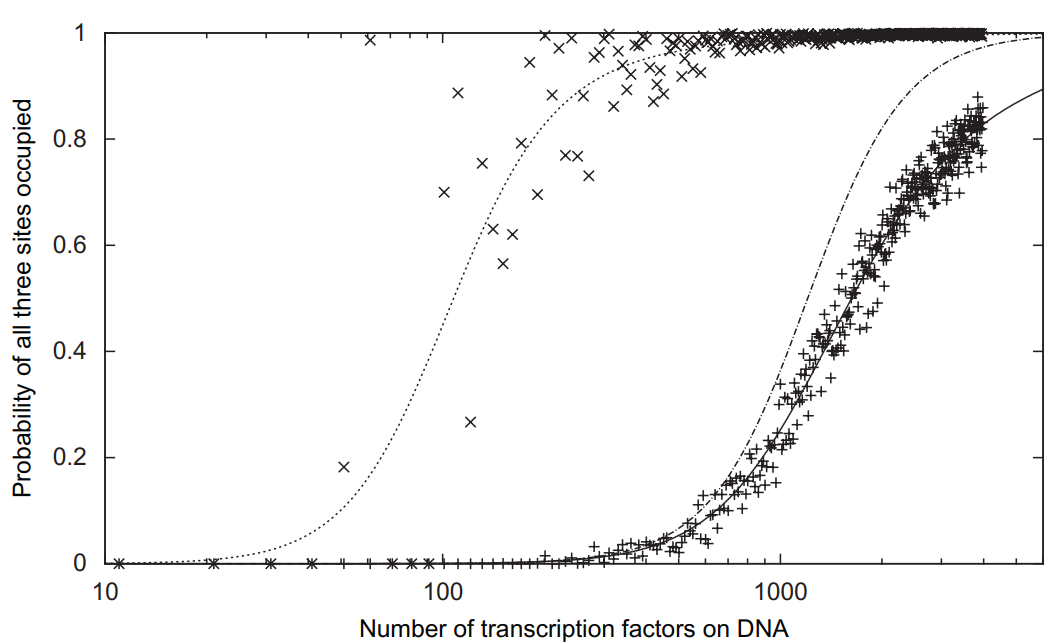
\includegraphics[width=7cm]{hill.png}
\caption{Hill approximation to stat mech based TF binding model}
\end{figure}
\end{textblock*}

\end{frame}



\begin{frame}{A scalable algorithm for inferring gene regulatory networks}

Interest in reverse-engineering whole-genome interaction networks from simultaneous measurements of the
expression levels of all (or at least most) genes in many
samples, under a common set of experimental conditions\\
\vspace{0.2in}
This algorithm applies when it is valid to assume that the system is in a steady state. For systems out of equilibrium, we need inference algorithms designed to operate on time-series data\\
\vspace{0.2in}
Typically gene expression data have low sampling rates and relatively small
amount of data. Moreover, GRNs have a high number of genes
with complex, nonlinear regulatory mechanisms

\end{frame}


\begin{frame}{Experimental considerations}

Gene interactions are inferred from gene expression data. RNA-seq has single cell-specificity and time resolution but lacks spatial resolution and data is noisy\\
\vspace{0.2in}
FISH techniques have single-cell specificity, spatial resolution, less noisy, but multiplexing is difficult and cells are fixed\\
\vspace{0.2in}

High cost of multiplexing precludes acquisition of time-resolved data is single cell studies, which is important when statistics of the genes of interest are not stationary (circadian rhythms, cell-cycle, drug-treatment.\\
\vspace{0.2in}

Transcription is not necessarily Poisson-like and has been shown to have switching behavior (transcriptional bursts). This has important implications for our models\\
\vspace{0.2in}

Even when we can collect single-cell time-series data, data collected at a time point will contain extra variability due to asynchrony of cells within a population (in terms of progression through a biological process)\\

\end{frame}

\begin{frame}{The Phi-Mixing Coefficient}

Interest in reverse-engineering whole-genome interaction networks from simultaneous measurements of the
expression levels of all (or at least most) genes in many
samples, under a common set of experimental conditions\\
\vspace{0.2in}
This algorithm applies when it is valid to assume that the system is in a steady state. For systems out of equilibrium, we need inference algorithms designed to operate on time-series data\\
\vspace{0.2in}
Typically gene expression data have low sampling rates and relatively small
amount of data. Moreover, GRNs have a high number of genes
with complex, nonlinear regulatory mechanisms

\end{frame}

\section{References}

\begin{frame}{Important topics}

Models range from networks of a few genes with detailed dynamical models to very large networks with coarse statistical description.
\vspace{0.2in}

\begin{itemize}
\item Linear dynamics of small networks (deterministic, stochastic)
\item Nonlinear dynamics of small networks (deterministic, stochastic) - Bintu model
\item Inferring network structure - Phi-Mixing Coefficient
\item Inferring network structure from linear dynamics - Hidden Markov Models
\item Inferring nonlinear network structure from empirical data - ?
\item Simulating stochastic dynamics (Gillespie algorithm)
\item Simulating stochastic nonlinear dynamics (Michaelis-Menten kinetics, SERGIO)
\item Transcriptional bursting - switching behavior of gene promoter
\end{itemize}


\end{frame}

% Adding the option 'allowframebreaks' allows the contents of the slide to be expanded in more than one slide.
\begin{frame}[allowframebreaks]{References}
	\tiny\bibliography{references}
	\bibliographystyle{apalike}
\end{frame}

\end{document}
